\documentclass{article}

\usepackage{preamble}

\title{Causality in Event Structure}
\author{Amir Hossein Seyhani}
\date{June 2022}

\begin{document}

\maketitle

\tableofcontents
\pagebreak

\section{Introduction}

\section{Preliminaries}
\subsection{Event Structure}
\begin{definition}[Event Structure]
    An event structure is a triple $E = (\mathcal{E},\#,\vdash)$ where:
    \begin{enumerate}
        \item $\mathcal{E}$ is a set of events
        \item \# is a binary symmetric, irreflexive relation on $\mathcal{E}$,
              the conflict relation.
              We shall write $Con$ for the set of conflict-free subsets of $\mathcal{E}$,
              i.e. those finite subsets $X \subseteq \mathcal{E}$ for which:
              $\forall e,e' \in X . \neg (e\#e')$
        \item $\vdash \subseteq Con \times \mathcal{E}$ is the enabling relation which satisfies:
              $ X \vdash e \ \& \ X \subseteq Y \in Con \Rightarrow Y \vdash e$
    \end{enumerate}

\end{definition}
\begin{notion}
    In an event structure we shall write $\doublevee$ for the reflexive conflict relation by which we mean
    that $e\doublevee e'$ in an event structure iff either $e\#e'$ or $e=e'$.
    With this notion instead of describing the conflict-free sets of an event structure
    as those sets $X$ such that
    \begin{align*}
        \forall e,e' \in X. \neg(e\#e')
    \end{align*}
    we can say they are those sets $X$ for which:
    \begin{align*}
        \forall e,e' \in X. e\doublevee e' \Rightarrow e=e'
    \end{align*}
\end{notion}

\begin{notion}
    For any event structure we can define the minimal enabling relation $\vdash_{min}$ by:
    \begin{align*}
        X \vdash_{min} e \iff X \vdash e \amp
        ( \forall Y \subseteq X . Y \vdash e \Rightarrow Y = X )
    \end{align*}
    Then for any event structure:
    \begin{align*}
        Y \vdash e \Rightarrow \exists X \subseteq Y . X \vdash_{min} e
    \end{align*}
\end{notion}

\begin{definition}[Configuration]
    \label{conf}
    Let $E = (\mathcal{E},\#,\vdash)$ be an event structure.
    Define a configuration of $E$ to be a subset of events $x \subseteq \mathcal{E}$ which is
    \begin{enumerate}
        \item conflict-free: $x \in Con$
        \item secured: $\forall e \in x \exists e_0,...,e_n \in x. e_n = e \ \& \
                  \forall i \leq n. \s{e_0,...,e_{i-1}} \vdash e_i$
    \end{enumerate}
\end{definition}
The set of all configurations of an event structure is written as $\mathcal{F(E)}$.
It is helpful to unwrap condition (2) a little. It says an event $e$ is secured in a set $x$
iff there is a sequence of events $e_0,...,e_n = e$ in $x$ such that:
\begin{align*}
    \emptyset \vdash e_0, \s{e_0} \vdash e_1, ..., \s{e_0,...,e_{i-1}} \vdash e_i,...,
    \s{e_0,...,e_{n-1}} \vdash e_n.
\end{align*}
We call such a sequence $e_0,e_1,...,e_n = e$ a \emph{securing} for $e$ in $x$.
We use $X \subseteq_{fin} Y$ to mean $X$ is a finite subset of $Y$.

\begin{example}
    Consider a network with two hosts $h_1$ and $h_2$ that are
    connected to a single switch.
    Assume that a packet arrives at the switch and then the switch
    non-deterministically forwards the packets to either $h_1$ or $h_2$.
    \begin{center}
        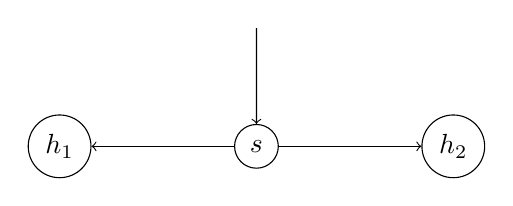
\begin{tikzpicture}[node distance={25mm},main/.style = {draw, circle}]
            \node[main] (H1) {$h_1$};
            \node[main] (S) [right of=H1] {$s$};
            \node[main] (H2) [right of=S] {$h_2$};
            \draw[<-] (H1) -- (S);
            \draw[->] (S) -- (H2);
            \draw[<-] (S) -- (2.5,1.5);
        \end{tikzpicture}
    \end{center}
    To model this scenario in event structures we can define an event
    $p$ for the arrival of the packet at the switch and events $h_1$
    and $h_2$ for the forwarding the packet to the hosts.
    The enabling relation is the least one for which we have:
    \begin{align*}
        \emptyset \vdash_{min} s,
        \s{s} \vdash_{min} h_1,
        \s{s} \vdash_{min} h_2,
    \end{align*}
    And we consider the conflict relation the least one that satisfies
    $h_1 \# h_2$.
    We illustrate configurations of event structures using the Hasse diagram of
    the partial order of configurations ordered by inclusion:
    \begin{center}
        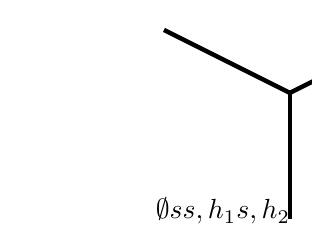
\begin{tikzpicture}[scale=0.8]
            \crd[right]{0}{0}{$\emptyset$}
            \crd{0}{2}{$\s{s}$}
            \crd{-2}{3}{$\s{s,h_1}$}
            \crd{2}{3}{$\s{s,h_2}$}
            \draw [ultra thick] (0,0) -- (0,2);
            \draw [ultra thick] (0,2) -- (-2,3);
            \draw [ultra thick] (0,2) -- (2,3);
        \end{tikzpicture}
    \end{center}
    We can see that non-determinism appears as branching in the partial order of configurations.
\end{example}

\begin{example}
    Consider another network in which two hosts are connected
    to a single switch.
    This time both hosts are sending a packet concurrently to the
    host.
    Once the switch received a packet from either host it will
    drop the packets received from the other host due to capacity
    limit.
    \begin{center}
        \begin{tikzpicture}[node distance={15mm},main/.style = {draw, circle}]
            \node[main] (S) [right of=H1] {$s$};
            \node[main] (H1) [above of=S,left of=S] {$h_1$};
            \node[main] (H2) [above of=S,right of=S] {$h_2$};
            \draw[->] (H1) -- (S);
            \draw[<-] (S) -- (H2);
        \end{tikzpicture}
    \end{center}
    Let $r_1,r_2$ represent the events of receiving packet from
    $h_1$ and $h_2$ and $d_1,d_2$ represent the events of dropping
    packets from these hosts.
    We need a conflict relation the least one for which we have
    $r_1\#d_1$ and $r_2\#d_2$
    and enabling relation the least one that satisfies:
    \begin{align*}
        \emptyset & \vdash_{min} r_1 \\
        \emptyset & \vdash_{min} r_2 \\
        \s{r_1}   & \vdash_{min} d_2 \\
        \s{r_2}   & \vdash_{min} d_1 \\
    \end{align*}
    Thus the configurations have the form:
    \begin{center}
        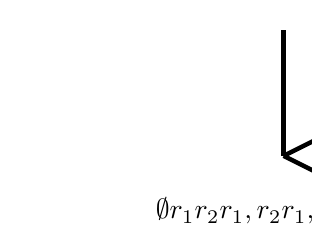
\begin{tikzpicture}[scale=0.8]
            \crd{0}{0}{$\emptyset$}
            \crd[left]{-2}{1}{$\s{r_1}$}
            \crd[right]{2}{1}{$\s{r_2}$}
            \crd[right]{0}{2}{$\s{r_1,r_2}$}
            \crd{-2}{3}{$\s{r_1,d_2}$}
            \crd{2}{3}{$\s{r_2,d_1}$}
            \draw [ultra thick] (0,0) -- (2,1);
            \draw [ultra thick] (0,0) -- (-2,1);
            \draw [ultra thick] (-2,1) -- (0,2);
            \draw [ultra thick] (2,1) -- (0,2);
            \draw [ultra thick] (-2,1) -- (-2,3);
            \draw [ultra thick] (2,1) -- (2,3);
        \end{tikzpicture}
    \end{center}
\end{example}

\begin{example}
    Consider two parallel switches in a circuit where they are connected
    to a light bulb.
    An event may be enabled in more than one way even in a single configuration.
    Assume initially both switches are open.
    Closing either one enables the event of the bulb lighting up.
    The configurations have the form:

    \begin{center}
        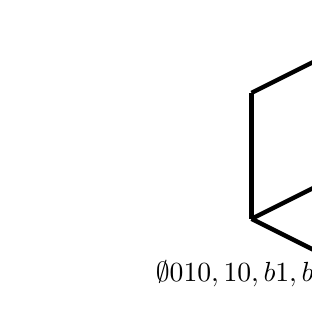
\begin{tikzpicture}[scale=0.8]
            \crd{0}{0}{$\emptyset$}
            \crd[left]{-2}{1}{$\s{0}$}
            \crd[right]{2}{1}{$\s{1}$}
            \crd[right]{0}{2}{$\s{0,1}$}
            \crd{-2}{3}{$\s{0,b}$}
            \crd{2}{3}{$\s{1,b}$}
            \crd{0}{4}{$\s{0,1,b}$}
            \draw [ultra thick] (0,0) -- (2,1);
            \draw [ultra thick] (0,0) -- (-2,1);
            \draw [ultra thick] (-2,1) -- (0,2);
            \draw [ultra thick] (2,1) -- (0,2);
            \draw [ultra thick] (-2,1) -- (-2,3);
            \draw [ultra thick] (0,2) -- (0,4);
            \draw [ultra thick] (2,1) -- (2,3);
            \draw [ultra thick] (-2,3) -- (0,4);
            \draw [ultra thick] (2,3) -- (0,4);
        \end{tikzpicture}
    \end{center}
\end{example}

We look for a special class of event structures for which there is a
partial order of causal dependency on each configuration.
This can not be done so obviously for all event structures.
Consider the event structure of the previous example in which
the event $b$ causally depends not on a unique set of events
but rather on either the occurrence of 0 or on the occurrence of 1.
It is incorrect to say $b$ causally depends on both 0 and 1 because
the occurrence of only one of them enables the occurrence of $b$.
The difficulty arises because there is a configuration $\s{0,1,b}$
in which there is an event $b$ which is not enabled by a unique minimal
set of event occurrences.
We can rule out such possibilities by insisting event structures
satisfy the following stability axiom.

\begin{definition}[Stable Event Structure]
    Let $E = (\mathcal{E},\#,\vdash)$ be an event structure. Say $E$ is stable if it satisfies the following axiom:
    \begin{align*}
        X \vdash e \ \& \ Y \vdash e \ \& \ X \cup Y \cup \{e\} \in Con \Rightarrow X \cap Y \vdash e
    \end{align*}
\end{definition}

The stability axiom ensures that an event in a configuration is
enabled in an essentially unique way.
Assume $e$ belongs to a configuration $x$ of a stable event structure.
Suppose $X \vdash e$ and $X \subseteq x$.
Then $X \cup \s{e} \in Con$, the enabling $X\vdash e$ is consistent.
Take
\begin{align*}
    X_0 = \cap \s{Y | Y \subseteq X \amp Y \vdash e}
\end{align*}
Because $X$ is finite this is an intersection of a finite number of
sets and we see by the stability axiom that $X_0 \vdash e$.
Moreover $X_0$ is the unique minimal subset of $X$ which enables $e$.
Thus for stable event structures, we have:
\begin{align*}
    Y \vdash e \amp Y \cup \s{e} \in Con \Rightarrow
    \exists ! X \subseteq Y.X \vdash_{min} e
\end{align*}
It follows that for stable event structures
\begin{align*}
    X \vdash_{min} e \amp Y \vdash_{min} \amp
    X \cup Y \cup e \in Con \Rightarrow X = Y
\end{align*}

\begin{theorem}
    Let $E = (\mathcal{E}, \#, \vdash)$ be an event structure.
    Let $x = \s{e_1,e_2,...,e_n}$ be a conflict-free subset of $\mathcal{E}$.
    Then $x$ is secured according to the definition \ref{conf} iff
    there exists an event $e_{i_n} \in x$ with a securing sequence $e_{i_1},e_{i_2},...,e_{i_{n-1}}$.
\end{theorem}
\begin{proof}
    Let $x$ be secured.
    We construct a securing sequence of length $n$.
    Pick two arbitrary events $e, e' \in x$.
    Since $x$ is secured there exists some securing sequences
    $s = e_{i_1},e_{i_2},...,e_{i_m}$
    and $s' = e_{i'_1},e_{i'_2},...,e_{i'_{m'}}$
    for $e$ and $e'$ respectively where $e_{i_m} = e$
    and $e_{i_{m'}'} = e'$.
    For $1 \leq a \leq b \leq p$,
    let $s'' = e_{j_1},e_{j_2},...,e_{j_p}$
    be the sequence resulting from appending $s'$ to $s$.
    Let $es(a,b) = \s{e_{j_a},e_{j_{a+1}},...,e_{j_{b}}}$.
    Pick an arbitrary event $e_{j_q}$ with $q > m$.
    In order for $s''$ to be a securing sequence, we must have
    $es(1,j_{p-1}) \vdash e_{j_p}$.
    Since we have $es(j_{m+1},j_{p-1}) \vdash e_{j_p}$ and
    $es(j_{m+1},j_{p-1}) \subseteq es(1,j_{p-1})$ thus we can conclude
    that $es(1,j_{p-1}) \vdash e_{j_p}$.
    Now assume that there exists an event such as $e_{j_q}$ with $q > m$ for which we have $\exists q'. q' \leq m \wedge j_{q'} = j_q$.
    Let $es'(1,j_{p-1})$ be the set of events preceding $e_{j_p}$, if we remove $e_{j_q}$ from $s''$.
    We still have $e_{j_{q'}} \in es'(1,j_{p-1})$ thus we can conclude that $es'(1,j_{p-1}) = es(1,j_{p-1})$ so $es'(1,j_{p-1}) \vdash e_{j_{p}}$.
    So, we can remove any duplicate event after $e_{j_m}$ and still
    have a securing sequence.
    This proves that we can construct a securing sequence by
    appending the securing sequence of two arbitrary events.
    So, we can first pick two arbitrary events and construct the
    resulting securing sequence and then repeat this procedure until
    we construct the full securing sequence.

    Now assume that there exists an event $e_{i_n}$ with a securing
    sequence $e_{i_1},e_{i_2},...,e_{i_{n-1}}$.
    Regarding the definition of securing sequence each event has a
    securing sequence, thus $x$ is secured.
\end{proof}

\begin{definition}
    Let $E_0 = (\mathcal{E}_0,\#_0,\vdash_0)$ and $E_1 = (\mathcal{E}_1,\#_1,\vdash_1)$
    be event Structures. Define
    \begin{align*}
        E_0 \trianglelefteq E_1 \iff & \mathcal{E}_0 \subseteq \mathcal{E}_1,                                          \\
                                     & \forall e,e'. e\#_0e'  \iff e,e' \in \mathcal{E}_0 \ \& \ e\#_1 e' \text{ and } \\
                                     & \forall X,e.X\vdash_0 e  \iff X \subseteq \mathcal{E}_0
        \ \& \ e \in \mathcal{E}_0\ \& \ X \vdash_1 e
    \end{align*}
    In this case say $E_0$ is a substructure of $E_1$.
\end{definition}

\begin{definition}[Restriction]
    Let $E = (\mathcal{E},\#,\vdash)$ be an event structure.
    Let $A \subseteq \mathcal{E}$.
    Define the restriction of $E$ to $A$ to be
    \begin{align*}
        E \lceil A = (A,\#_A,\vdash_A)
    \end{align*}
    where
    \begin{align*}
        X \in Con_A \iff X \subseteq A \ \& \ X \in Con \\
        X \vdash_A e \iff X \subseteq A \ \& \ e \in A \ \& \ X \vdash e
    \end{align*}
\end{definition}

\begin{definition}
    Let $a$ be an event.
    For an event structure $E = (\mathcal{E},\#,\vdash)$ define $aE$ to be the event structure $(\mathcal{E'},\#',\vdash')$ where:
    \begin{align*}
         & \mathcal{E'} = \s{(0,a)} \cup \s{(1,e)|e \in \mathcal{E}},                                                   \\
         & e_0' \#' e_1'  \iff \exists e_0,e_1.e_0' = (1,e_0)
        \ \& \ e_1' = (1,e_1) \ \& \ e_0 \# e_1                                                                         \\
         & X \vdash' e' \iff e' = (0,a) \text{ or } [e' = (1,e_1) \ \& \ (0,a)\in X \ \& \ \s{e|(1,e)\in X} \vdash e_1]
    \end{align*}
\end{definition}

\begin{definition}
    A labelled event structure consists of $(\mathcal{E},\#,\vdash,L,l)$ where
    $(\mathcal{E},\#,\vdash)$ is an event structure, $L$ is a set of labels,
    not including the element *, and $l$ is a function $l: \mathcal{E} \rightarrow L$
    from its events to its labels.
\end{definition}
\begin{notion}
    We write $(a_1,a_2,...,a_{n-1},a_n)$ to denote the event:
    \begin{align*}
        e = (a_1,(a_2,(a_3,...(a_{n-1},a_n))))
    \end{align*}
\end{notion}

\subsection{Causal Model}

A signature $\mathcal{S}$ is a tuple $(\mathcal{U},\mathcal{V},\mathcal{R})$,
where $\mathcal{U}$ is a set of exogenous variables, $\mathcal{V}$
is a set of endogenous variables, and $R$ associates with every variable
$Y\in \mathcal{U}\cup \mathcal{V}$ a nonempty set $\mathcal{R}(Y)$ of possible values for $Y$.
A causal model (or structural model) over signature $S$ is a tuple
$M=(\mathcal{S},\mathcal{F})$, where $\mathcal{F}$ associates with
each variable $X \in \mathcal{V}$ a function denoted $F_X$ such that
$F_X: (\times_{U\in \mathcal{U}}\mathcal{R}(U))\times (\times_{Y\in\mathcal{V}-\{X\}}\mathcal{R}(Y))\rightarrow \mathcal{R}(X)$.

$F_X$ determines the value of $X$ given the values of all the other variables
in $\mathcal{U}\cup \mathcal{V}$.
For example, if $F_X(Y,Z,U)=Y+U$ (which we usually write as $X = Y + U$),
then if $Y=3$ and $U=2$, then $X = 5$, regardless of how $Z$ is set.
These equations can be thought of as representing processes (or mechanisms) by which values are assigned to variables. Hence, like physical laws, they support a counterfactual interpretation.
For example, the equation above claims that in the context $U=u$, if $Y$ were 4, then $X$ would be $u+4$ (which we write as $(M,u) \models [Y\leftarrow 4](X = u + 4))$, regardless of what values X, Y, and Z actually take in the real world.


The function $\mathcal{F}$ defines a set of (\textit{modifiable}) \textit{structural equations} relating to the values of the variables.


\subsection{Definition of Actual Cause}
Given a signature $S= (\mathcal{U},\mathcal{V},\mathcal{R})$, a formula of the form $X =x$, for $X \in \mathcal{V}$ and $x \in \mathcal{R}(X)$, is called a \textit{primitive event}.
A \textit{basic causal formula} is one of the form $[Y_1 \leftarrow y_, ..., Y_l\leftarrow y_k]\varphi$, where $\varphi$ is a Boolean combination of primitive events, $Y_1,...,Y_k$ are distinct variables in $\mathcal{V}$, and $y_i \in \mathcal{R}(Y_i)$.
Such a formula is abbreviated as $[\vec{Y}\leftarrow\vec{y}]\varphi$.
A \textit{causal formula} is a Boolean combination of basic causal formulas.
A causal formula $\psi$ is true or false in a causal model, given a context.
We write $(M,\vec u)\models \psi$ if $\psi$ is true in causal model $M$ given context $\vec u$.
$(M,\vec u)\models [\vec Y\leftarrow \vec y](X=x)$ if the variable $X$ has value $x$ in the unique solution to the equation in $M_{\vec{Y} \leftarrow \vec{y}}$ in context $\vec u$.
The context and structural equations are given.
They encode the background knowledge.
All relevant events are known.
The only question is picking out which of them are the cause of $\varphi$ or, alternatively, testing whether a given set of events can be considered the cause of $\varphi$.
The types of events that we allow as actual causes are ones of the form $X_1 = x_1 \wedge ... \wedge X_k=x_k$-- that is, conjunctions of primitives events.
We abbreviate this as $\vec X = \vec x$.
\\
\\
\begin{definition}

    $\vec X = \vec x$ is an actual cause of $\varphi$ in $(M,\vec u)$ if the following three conditions hold:
    \begin{itemize}
        \item  \textbf{AC1.} $(M,\vec u)\models (\vec X = \vec x) \wedge \varphi$.
              (both $\vec X = \vec x$ and $\varphi$ are true in actual world)
        \item  \textbf{AC2. }There exists a partition $(\vec Z, \vec W)$ of $\mathcal{V}$ with $\vec X \subseteq \vec Z$ and some setting $(\vec x',\vec w')$ of the variables in $(\vec X,\vec W)$ such that if $(M,\vec u)\models \vec Z = z^*$ for all $Z\in \vec Z$, then both of the following conditions hold:

              (a) $(M,\vec u)\models[\vec X \leftarrow \vec x', \vec W \leftarrow \vec w']\neg \varphi$.

              (b) $(M,\vec u)\models[\vec X\leftarrow \vec x, \vec W' \leftarrow \vec w', \vec Z'\leftarrow \vec z^*]\varphi$ for all subsets $\vec W'$ of $\vec W$ and all subsets $Z'$ of $\vec Z$.

        \item  \textbf{AC3.} $\vec X$ is minimal; no subset of $\vec X$ satisfies conditions $AC1$ and $AC2$.
    \end{itemize}
\end{definition}
We call the tuple $(\vec W, \vec w,\vec x')$ a witness to the fact that $\vec X=\vec x$ is a cause of $\varphi$.

\begin{definition}
    We say $\vec X = \vec x$ is a but-for cause of $\varphi$ in
    $(M,\vec u)$ if there exists a witness $(\vec W, \vec w, \vec x')$
    for $\vec X = \vec x$ where $\vec W = \emptyset $.
\end{definition}

Note that, if we consider a witness $(\vec W, \vec w, \vec x')$
for checking whether $\vec X = \vec x$ is a cause of $\varphi$
in $(M,\vec u)$ where $\vec W = \e$, then in the AC2(b) condition
we only need to check whether $(M,\vec u) \vDash [\vec X \leftarrow \vec x, \vec Z' \leftarrow \vec z^*]\varphi$ for all subsets $\vec Z'$
of $\vec Z$.
Since we have $(M,\vec u) \vDash (\vec X = \vec x)$ and
$(M,\vec u) \vDash Z = z^*$ for all $Z \in vec Z$,
the Interventions $\vec X \leftarrow \vec x$ and
$\vec Z ' \leftarrow \vec z^*$ actually do not change the value of
any variable thus checking whether
$(M,\vec u) \vDash [\vec X \leftarrow \vec x, \vec Z' \leftarrow \vec z^*]\varphi$ is true
reduces to check whether $(M,\vec u) \vDash \varphi$
which must be already satisfied when we have checked AC1 condition.
This means that, to check whether $\vec X = \vec x$ is an actual cuase when using a witness with an empty $\vec W$
we only need to check AC1 and AC2(a) conditions.

\subsection{Actual Cause in Non-Recursive Models}

\newcommand{\la}{\leftarrow}
In non-recursive models, there may be more than one solution to
an equation in a given context, or there may be none.
In particular, that means that a context no longer necessarily
determines the values of endogenous variables.
We identified a primitive event such as $X = x$ with basic causal formula $[](X=x)$, that is, with the special case of a formula
of the form $[Y_1 \la y_1,...,Y_k\la y_k ]\varphi$ with $k =0 $.
We say $(M,\vec u) \vDash [] (X = x)$ if $X=x$ in all solutions
to the equations where $\vec U = \vec u$.
If seems reasonable to identify $[](X=x)$ with $X=x$ if there
is a unique solution to these equations.
But it is not so reasonable if there may be several solutions,
or no solution.
What we really want to do is to be able to say that $X=x$ under
a particular setting of variables.
Thus, we now take the truth of a primitive event such as $X=x$
relative not just to a context, but to a complete description
$(\vec u, \vec v)$ of the values of both the exogenous and
the endogenous variables.
That is, $(M,\vec u,\vec v) \vDash X =x$ if $X$ has value $x$ in $\vec v$.
Since truth value of $X=x$ depends on just $\vec v$, not $\vec u$,
we sometimes write $(M,\vec v) \vDash X =x$.
We then define $(M,\vec u, \vec v) \vDash[\vec Y \la \vec y]\varphi$ if $(M,\vec v') \vDash \varphi$ for all solutions
$(\vec u, \vec v')$ to the equations in $M_{\vec Y \la \vec y}$.
Since the truth of $[\vec Y \la \vec y](X=x)$ depends only on the
context $\vec u$ and not on $\vec v$, we typically write $(M,\vec u) \vDash[ \vec Y \la \vec y](X=x)$.

The formula $\langle \vec Y \la \vec y \rangle(X=x)$ is the dual
of $[\vec Y \la \vec y](X=x)$; that is, it is an abbreviation of
$\neg [\vec Y \la \vec y](X \neq x)$.
It is easy to check that
$(M,\vec u, \vec v) \vDash \langle \vec Y \la \vec y \rangle(X=x)$
if in some solution to the equations in $M_{\vec Y \la \vec y}$ in
context $\vec u$, the variable $X$ has value $x$.
For recursive models, it is immediate that
$[\vec Y \la \vec y](X = x)$ is equivalent to
$\langle \vec Y \la \vec y \rangle(X=x)$ since all equations
have exactly one solution.
Now we can state the definition of causality for arbitrary models.
\begin{definition}
    $\vec X = \vec x$ is an actual cause of $\varphi$ in
    $(M,\vec u, \vec v) $ if the following three conditions hold.

    \begin{itemize}
        \item  \textbf{AC1.} $(M,\vec v)\models (\vec X = \vec x) \wedge \varphi$.
        \item  \textbf{AC2. }There exists a partition $(\vec Z, \vec W)$ of $\mathcal{V}$ with $\vec X \subseteq \vec Z$ and some setting $(\vec x',\vec w')$ of the variables in $(\vec X,\vec W)$ such that if $(M,\vec u, \vec v)\models \vec Z = z^*$ for all $Z\in \vec Z$, then both of the following conditions hold:

              (a) $(M,\vec u)\models \langle \vec X \leftarrow \vec x', \vec W \leftarrow \vec w' \rangle \neg \varphi$.

              (b) $(M,\vec u)\models[\vec X\leftarrow \vec x, \vec W' \leftarrow \vec w', \vec Z'\leftarrow \vec z^*]\varphi$ for all subsets $\vec W'$ of $\vec W$ and all subsets $Z'$ of $\vec Z$.

        \item  \textbf{AC3.} $\vec X$ is minimal; no subset of $\vec X$ satisfies conditions $AC1$ and $AC2$.
    \end{itemize}
\end{definition}

\subsection{Extended Causal Model}
An extended causal model is a tuple $(\mathcal{S},\mathcal{F},
    \mathcal{E})$, where $(\mathcal{S},\mathcal{F})$ is a causal model, and $\mathcal{E}$ is a set of allowable settings for the endogenous variables.
That is, if the endogenous variables are $X_1,...,X_n$ then
$(x_1,...,x_n) \in \mathcal{E}$ if $X_1 = x_1, ..., X_n=x_n$ is an
allowable setting.
We say that a setting of a subset of the endogenous variables is allowable if it can be extended to a setting in $\mathcal{E}$.
We then modify the clauses AC2(a) and (b) in the definition of causality to restrict to allowable settings.
Let $\psi$ be a function $(\times_{X \in \mathcal{V}}R(X))\rightarrow \mathbb{B}$ defined on the set of endogenous variables.
We define the model $(\mathcal{S},\mathcal{F},\psi)$ to be equal
to the model $(\mathcal{S},\mathcal{F},\mathcal{E})$ where
for each setting $\vec x$ of endogenous variables we have $\vec x \in \mathcal{E} \iff \psi(\vec x) = true$.
Thus, given an extended causal model $M = (\mathcal{S},\mathcal{F},\psi)$ we redefine the actual cause as follows:

\begin{definition}
    $\vec X = \vec x$ is an actual cause of $\varphi$ in $(M,\vec u)$ if the following three conditions hold:
    \begin{itemize}
        \item  \textbf{AC1.} $(M,\vec u)\models (\vec X = \vec x) \wedge \varphi \wedge \psi(\vec v)$.
        \item  \textbf{AC2. }There exists a partition $(\vec Z, \vec W)$ of $\mathcal{V}$ with $\vec X \subseteq \vec Z$ and some setting $(\vec x',\vec w')$ of the variables in $(\vec X,\vec W)$ such that if $(M,\vec u)\models \vec Z = z^*$ for all $Z\in \vec Z$, then both of the following conditions hold:

              (a) $(M,\vec u)\models[\vec X \leftarrow \vec x', \vec W \leftarrow \vec w']\neg \varphi \wedge \psi(\vec v)$.

              (b) $(M,\vec u)\models[\vec X\leftarrow \vec x, \vec W' \leftarrow \vec w', \vec Z'\leftarrow \vec z^*]\varphi \wedge \psi(\vec v)$ for all subsets $\vec W'$ of $\vec W$ and all subsets $Z'$ of $\vec Z$.

        \item  \textbf{AC3.} $\vec X$ is minimal; no subset of $\vec X$ satisfies conditions $AC1$ and $AC2$.
    \end{itemize}
\end{definition}

\section{Semantics of Communicating Processes}
One use of event structure is to give a denotational semantics of language of parallel
processes which reflects the parallelism in processes as causal independence between events.
The nature of the events, how they interact with the environment,
is specified in the language by associating each event with a label from the synchronization
algebra $L$.
The language we shall use is one where processes communicate by events of synchronization
with no value passing.
Its syntax has the form:
\begin{align*}
    p ::= nil | \alpha p | p_0 + p_1 | p_0 \times p_1 | p\lceil \Lambda | p[\Xi] | x | recx.p
\end{align*}
where $x$ is in some set of variables $X$ over processes, $\alpha$ is a label,
$\Lambda$ is a subset of labels, in $p[\Xi]$ the symbol $\Xi$ denotes a relabelling function between
two sets of labels.

Informally, the product $p_0 \times p_1$ is a form of parallel composition which introduces
arbitrary events of synchronization between process.
Unwanted synchronizations can be restricted away with the help of the restriction operation
$p\lceil \Lambda$ and the existing events renamed with the relabelling operation $p[\Xi]$.
So in this way we can define specialized parallel compositions of the kind that appear in
CCS and CSP, for example.
To explain formally the behavior of the constructs in the language we describe them as
constructions on labelled event structures, so a closed process term in this language is to
denote a \textbf{stable event structure} but where the events are labelled.

\subsection{Nil}
The term $nil$ represents the $nil$ process which has stopped and refuses to perform any event;
it will denoted by the empty labelled event structure $(\emptyset,\emptyset,\emptyset,\emptyset,\emptyset)$
no events, no labels.

\subsection{Prefix}

\begin{definition}
    Let $(\mathcal{E},L,l)$ be a labelled event structure.
    Let $\alpha$ be a label.
    Define $\alpha(\mathcal{E},L,l)$ to be a labelled event structure $(\alpha \mathcal{E},L',l')$
    with labels:
    \begin{align*}
        L' = \s{\alpha} \cup L
    \end{align*}
    and
    $$
        l'(e') = \begin{cases}
            \alpha & \text{if } e' = (0,\alpha) \\
            l(e)   & \text{if } e' = (1,e)
        \end{cases}
    $$
    for all $e' \in \mathcal{E'}$.
\end{definition}
The configurations of $\alpha E$, a prefixed labeled event structure,
have the simple and expected characterization.
(By $\mathcal{F}(E)$ of a labeled event structure $E$ we shall understand the set
of configurations of the underlying event structure)

\begin{proposition}

    Let $E$ be a labelled event structure. Let $\alpha$ be a label.
    \begin{align*}
        x \in \mathcal{F}(\alpha E) \iff x = \emptyset \text{ or }
        [(0,\alpha)\in x \amp \s{e | (1,e)\in x} \in \mathcal{F}(E)]
    \end{align*}

\end{proposition}

\subsection{Sum}
A sum $p_0 + p_1$ behaves like $p_0$ or $p_1$; which branch of a sum is followed will
often be determined by the context and what kinds of events the process is restricted to.

\begin{definition}
    Let $E_0 = (\mathcal{E}_0,\#_0,\vdash_0,L_0,l_0)$ and
    $E_1 = (\mathcal{E}_1,\#_1,\vdash_1,L_1,l_1)$ be labelled event structures.
    Their sum $E_0 + E_1$, is defined to be the structure $(\mathcal{E},\#,\vdash,l)$
    with events $\mathcal{E} = \s{(0,e)|e \in \mathcal{E}_0} \cup \s{(1,e)|e \in \mathcal{E}_1}$,
    the disjoint union of sets $\mathcal{E}_0$ and $\mathcal{E}_1$,
    with injections $\iota_k: \mathcal{E}_k \rightarrow \mathcal{E}$, given by
    $\iota_k(e) = (k,e)$, for $k=0,1$, conflict relation
    \begin{align*}
        e \# e' \iff & \exists e_0,e_0'. e = \iota_0(e_0)
        \amp e' = \iota_0(e_0') \amp e_0 \#_0e_0'                         \\
                     & \text{or } \exists e_1,e_1'. e = \iota_1(e_1) \amp
        e' = \iota_1(e_1') \amp e_1 \#_1 e_1'                             \\
                     & \text{or } \exists e_0,e_1.(e=\iota_1(e_0)
        \amp e' =\iota_1(e_1)) \text{ or }
        (e'=\iota_1(e_0) \amp e =\iota_1(e_1))
    \end{align*}
    and enabling relation
    \begin{align*}
        X \vdash e \iff & X \in Con \amp e \in \mathcal{E} \amp                       & \\
                        & (\exists X_0 \in Con_0,e_0 \in \mathcal{E}_0.X = \iota_0X_0
        \amp e = \iota_0(e_0) \amp X_0 \vdash_0 e_0) \text{ or }                        \\
                        & (\exists X_1 \in Con_1,e_1 \in \mathcal{E}_1.X = \iota_1X_1
        \amp e = \iota_1(e_1) \amp X_1 \vdash_1 e_1)                                    \\
    \end{align*}
    We define the set of labels as $L_0 \cup L_1$ and the labelling function as:
    $$
        l(e) = \begin{cases}
            l_0(e_0) & \text{ if } e = \iota_0(e_0) \\
            l_1(e_1) & \text{ if } e = \iota_1(e_1)
        \end{cases}
    $$
\end{definition}
The configurations of a sum are obtained from copies of the configurations of the components
identified at their empty configurations.

\begin{proposition}

    Let $E_0$ and $E_1$ be labelled event structures.
    \begin{align*}
        x \in \mathcal{F}(E_0+E_1) \iff (\exists x_0 \in \mathcal{F}(E_0).x=\iota_0x_0)
        \text{ or } (\exists x_1 \in \mathcal{F}(E_1).x=\iota_1x_1)
    \end{align*}

\end{proposition}

\subsection{Product}

A product process $p_0 \times p_1$ behaves like $p_0$ and $p_1$ set in parallel.
Their events of synchronization are those pairs of events $(e_0,e_1)$, one from each process;
if $e_0$ is labelled $\alpha_0$ and $e_1$ is labelled $\alpha_1$ the synchronization event is
then labelled $(\alpha_0,\alpha_1)$.
Events need not to synchronize however; an event in one component may not synchronize with
any event in the other.
We shall use events of the form $(e_0,*)$ to stand for the occurrence of an event $e_0$
from one component unsynchronized with any event of the other.
Such an event will be labelled by $(\alpha_0,*)$ where $\alpha_0$ is the original label of $e_0$
and * is a sort of undefined.

In fact we shall often want to take the first or second coordinates of such paris and,
of course, this could give the value * which we think of as undefined,
so that, in effect, we are working with partial functions with * understood to be undefined.
We can keep expressions tidier by adopting some conventions about how to treat this undefined value
when it appears in expressions and assertions.
\begin{align*}
     & \Theta(e) \in X \Rightarrow \Theta(e) \text{is defined, and }                                      \\
     & \Theta(e) = \Theta(e') \Rightarrow \Theta(e) \text{is defined } \amp \Theta(e')\text{ is defined}.
\end{align*}
We adopt a similar strict interpretation for function application.
So if $f$ is a function applied to some value, denoted by $a$, the $f(a)$ is undefined (gives *)
if $a$ is undefined.
As usual we represent the image of a set under a partial function by
\begin{align*}
    \Theta X = \s{\Theta(e)|e \in X \amp \Theta(e) \text{ is defined}}
\end{align*}

\begin{definition}

    Let $E_0 = (\mathcal{E}_0,\#_0,\vdash_0,L_0,l_0)$ and $E_1 = (\mathcal{E}_1,\#_1,\vdash_1,L_1,l_1)$
    be labelled event structures.
    Define their product $E_0 \times E_1$ to be the structure $E = (\mathcal{E},\#,\vdash,L,l)$
    consisting of events $\mathcal{E}$ of the form
    \begin{align*}
        \mathcal{E}_0 \times_* \mathcal{E}_1 =
        \s{(e_0,*)|e_0 \in \mathcal{E}_0}
        \cup \s{(*,e_1)|e_1 \in \mathcal{E}_1}
        \cup \s{(e_0,e_1)| e_0 \in \mathcal{E}_0 \amp e_1 \in \mathcal{E}_1}
    \end{align*}
    with projections $\pi_i : \mathcal{E} \rightarrow_* \mathcal{E}_i$,
    given by $\pi_i(e_0,e_1) = e_i$, for $i=0,1$, reflexive conflict relation $\doublevee$ given by
    \begin{align*}
        e \doublevee e' \iff \pi_0(e) \doublevee_0 \pi_0(e') \text{ or }
        \pi_1(e) \doublevee_1 \pi_1(e')
    \end{align*}
    for all $e,e'$ we use $Con$ for the conflict-free finite sets,
    enabling relation $\vdash$ given by
    \begin{align*}
         & X \vdash e \iff X \in Con \amp e \in \mathcal{E} \amp            \\
         & (\pi_0(e)\text{ is defined } \Rightarrow \pi_0X\vdash_0\pi_0(e))
        \amp (\pi_1(e)\text{ is defined } \Rightarrow \pi_1X\vdash_1\pi_1(e))
    \end{align*}
    Its set of labels is
    \begin{align*}
        L_0 \times_* L_1 = \s{ (\alpha_0,*)|\alpha_0 \in L_0}
        \cup \s{(*,\alpha_1)|\alpha_1 \in L_1}
        \cup \s{(\alpha_0,\alpha_1)|\alpha_0 \in L_0 \amp \alpha_1 \in L_1}
    \end{align*}
    with projections: $\lambda_i: \mathcal{E} \rightarrow_* \mathcal{E}_i$ given by
    $\lambda_i(\alpha_0,\alpha_1) = \alpha_i$, for $i=0,1$.
    Its labelling function is defined to act on an event $e$ so
    \begin{align*}
        l(e) = (l_0\pi_0(e),l_1\pi_1(e))
    \end{align*}
\end{definition}
We characterize the configurations of the product of two event structures in terms
of their configurations.

\begin{proposition}

    Let $E_0 \times E_1$ be the product of labelled event structures with projections
    $\pi_0,\pi_1$.
    Let $x \subseteq \mathcal{E}_0 \times \mathcal{E}_1$, the events of the product.
    Then $x \in \mathcal{F}(\mathcal{E}_0 \times \mathcal{E}_1)$ iff
    \begin{align*}
         & \pi_0(x)  \in \mathcal{F}(E_0) \amp \pi_1x \in \mathcal{F}(E_1)                                      \\
         & \forall e,e' \in x.\pi_0(e)=\pi_0(e') \text{ or } \pi_1(e) = \pi_1(e') \Rightarrow e = e'            \\
         & \forall e \in x \exists y \subseteq x. \pi_0 y \in \mathcal{F}(E_0) \amp \pi_1y \in \mathcal{F}(E_1)
        \amp e \in y \amp |y| < \text{infinite}                                                                 \\
         & \forall e,e' in x. e \neq e' \Rightarrow \exists y \subseteq x.\pi_0 y \in \mathcal{F}(E_0)
        \amp \pi_1y \in \mathcal{F}(E_1) \amp (e \in y \iff e' \not \in y)
    \end{align*}
\end{proposition}
The Proposition above expresses the intuition that an allowable behavior of the product
of two processes is precisely that which projects to allowable behaviors in the component
processes.
The complicated-looking conditions (c) and (d) are there just to ensure that the family
of sets is finitary and coincidence-free.

\subsection{Restriction}

The restriction $t \lceil \Lambda$ behaves like the process $p$ but with its events
restricted to those with labels which lie in the set $\Lambda$.

\begin{definition}

    Let $E = (\mathcal{E},\#,\vdash,L,l)$ be a labelled event structure.
    Let $\Lambda$ be a subset of labels.
    Define the restriction $E\lceil \Lambda$ to be $(\mathcal{E'},\#',\vdash',L\cap \Lambda,l')$
    where $(\mathcal{E'},\#',\vdash')$ is the restriction of $(\mathcal{E},\#,\vdash)$
    to events $\s{e \in \mathcal{E}|l(e) \in \Lambda}$ and the labelling function $l'$
    is the restriction of the original labelling function to the domain $L \cap \Lambda$.

\end{definition}

\begin{proposition}

    Let $E = (\mathcal{E},\#,\vdash,L,l)$ be a labelled event structure.
    Let $\Lambda \subseteq L$.
    \begin{align*}
        x \in \mathcal{F}(E\lceil\Lambda) \iff x \in \mathcal{F}(E) \amp e \in x.l(e) \in \Lambda
    \end{align*}

\end{proposition}

\subsection{Relabelling}

A relabelled process $p[\Xi]$ behaves like $p$ but with the events relabelled according to $\Xi$.

\begin{definition}

    Let $E = (\mathcal{E},\#,\vdash,L,l)$ be a labelled event structure.
    Let $\Lambda,L'$ be sets of labels and $\Xi: \Lambda \rightarrow L'$.
    Define the relabelling $E[\Xi]$ to be $(\mathcal{E},\#,\vdash,L',l')$ where
    $$
        l'(e) = \begin{cases}
            \Xi l(e) & \text{if } l(e) \in \Lambda \\
            l(e)     & \text{otherwise}
        \end{cases}
    $$

\end{definition}
\subsection{Denotational Semantics}

\begin{definition}
    Define an environment for process variables to be a function $\rho$
    from process variables $X$ to labelled event structures.
    For a term $t$ and environment $\rho$, define the denotation of $t$ with
    respect to $\rho$ written $\llbracket t \rrbracket \rho$ by the following
    structural induction syntactic operators appear on the left and their
    semantics counterparts on the right.
    \begin{equation*}
        \begin{aligned}[c]
            \sem{nil}\rho       & = (\emptyset,\emptyset)         \\
            \sem{x}\rho         & = \rho(x)                       \\
            \sem{\alpha t}\rho  & = \alpha(\sem{t}\rho)           \\
            \sem{t_1 + t_2}\rho & = \sem{t_1}\rho + \sem{t_2}\rho \\
        \end{aligned}
        \qquad
        \begin{aligned}[c]
            \sem{t\lceil \Lambda}\rho & = \sem{t}\rho \lceil \Lambda         \\
            \sem{t[\Xi]}\rho          & = \sem{t}\rho[\Xi]                   \\
            \sem{t_1 \times t_2}\rho  & = \sem{t_1}\rho \times \sem{t_2}\rho \\
            \sem{recx.t}\rho          & = fix\Gamma                          \\
        \end{aligned}
    \end{equation*}
    where $\Gamma$ is an operation on labelled event structures given by
    $\Gamma(E) = \sem{t}\rho[E / x]$ and $fix$ is the least-fixed-point operator.
\end{definition}

\section{Causality in Event Structure}
Let $E = (\mathcal{E},\#,\vdash,l,L)$ be an event structure with
$\mathcal{E} = \s{e_1, e_2, ...,e_n}$ and let $\s{s_1,s_2,...,s_p}$ be the power set of $\mathcal{E}$ where $p = 2^n$.
Without the loss of generality let $\sigma = \s{e_1,e_2,...,e_m}$ be a configuration of $E$ that
has been given as a counterexample.
To find the cause of this counterexample, first we construct an extended causal model $M = (\mathcal{S},\mathcal{F},\psi)$.
To define the signature $\mathcal{S} = (\mathcal{U},\mathcal{V},\mathcal{R})$, we assume that all variables in $\mathcal{U} \cup \mathcal{V}$ as a boolean variable.
Next, we define $\mathcal{U}$ and $\mathcal{V}$ as follows:
\begin{align*}
    \mathcal{U} = & \s{CE_{i,j} | \forall 1 \leq i < j \leq n. e_i \in \mathcal{E} \amp e_j \in \mathcal{E}}                    \\
                  & \cup \s{ME_{k,i} | \forall 1 \leq k \leq p , \forall 1 \leq i \leq n . s_k \in P \amp e_i \in \mathcal{E} } \\
    \mathcal{V} = & \s{C_{i,j} | \forall 1 \leq i < j \leq n. e_i \in \mathcal{E} \amp e_j \in \mathcal{E}}                     \\
                  & \cup \s{E_{k,i} | \forall 1 \leq k \leq p , \forall 1 \leq i \leq n . s_k \in P \amp e_i \in \mathcal{E} }  \\
                  & \cup \s{M_{k,i} | \forall 1 \leq k \leq p , \forall 1 \leq i \leq n . s_k \in P \amp e_i \in \mathcal{E} }  \\
\end{align*}
We define $\psi$ such that we can prevent invalid settings of variables:
\begin{align*}
    \psi(\vec v) = & \forall_{k,i}.
    \left(
    M_{k,i} \Rightarrow E_{k,i}
    \right)
    \wedge
    \left(
    E_{k,i} \Rightarrow Con(k)
    \right)
    \\
                   & \wedge \left(E_{k,i} \Rightarrow
    \forall k'. (s_k \subset s_{k'} \wedge Con(k')) \Rightarrow E_{k',i}
    \right)                                           \\
                   & \wedge \left(
    M_{k,i} \Rightarrow \forall k'.
    (s_{k'} \subset s_k) \Rightarrow \neg M_{k',i}
    \right)
\end{align*}
We consider the given event structure as a background knowledge.
Thus, we set value of the variables in $\mathcal{U}$ regarding
the given event structure.
Formally, we assume that:
\begin{align*}
    CE_{i,j} = \text{true} & \iff e_i \# e_j \wedge e_j\# e_i \\
    ME_{i,j} = \text{true} & \iff s_k \vdash_{min} e_i
\end{align*}
For $x,y \in \mathcal{P}(\mathcal{E})$ we say $y$ is covered by $x$ written $ x \prec y$ iff:
\begin{align*}
    x \subseteq y \amp x \neq y \amp
    (\forall z. x \subseteq z \subseteq y \Rightarrow x = z
    \text{ or } y = z)
\end{align*}
For each variable $x \in \mathcal{V}$ we define $\vec V_x$ as a vector
of all variables in $\mathcal{V}$ excluding $x$.
Let $\vec u$ be a setting of exogenous variables.
We define the functions in $\mathcal{F}$ as follows:
\begin{align*}
    Con(k)                                & =   \left(
    \bigwedge_{\forall j,j'. j<j' \amp e_j,e_{j'} \in s_k}
    \neg C_{j,j'}
    \right)                                                                          \\
    Min(k,i)                              & = \left(
    \bigwedge_{
        \forall k'. e_i \notin{s_{k'} \wedge \left(
            s_{k} \subset s_{k'} \vee s_{k'} \subset s_{k}
            \right)}
    } \neg M_{k',i}
    \right)                                                                          \\
    F_{C_{i,j}}(\vec u, \vec V_{C_{i,j}}) & = CE_{i,j}                               \\
    F_{M_{k,i}}(\vec u, \vec V_{M_{k,i}}) & = ME_{k,i} \wedge Min(k,i) \wedge Con(k) \\
    F_{E_{k,i}}(\vec u, \vec V_{E_{k,i}}) & =
    \left(
    M_{k,i} \vee
    \left(
    \bigvee_{\forall l. s_l  \prec s_k}E_{l,i}
    \right)
    \right)
    \bigwedge
    Con(k)
\end{align*}
With this causal model in hand, we define $\varphi_{\sigma}$ to represent whether $\sigma$ is a configuration of $E$.
To do this we need to encode the conflict-free and secured conditions in the definition \ref{conf}.
Let the sequence $\pi = e_{i_1},e_{i_2},...,e_{i_m}$ be a
permutation of events in $\sigma$ and $\mathcal{S}$ be the set of
all permutations of $\sigma$.
We define the following auxiliary functions:
\begin{align*}
    CE(e,e') = CE_{i,j}  & \iff e = e_i \wedge e' = e_j \\
    ME(s,e)  = ME_{k,i}  & \iff s = s_k \wedge e = e_i  \\
    C(e,e') = C_{i,j}    & \iff e = e_i \wedge e' = e_j \\
    M(s,e)  = M_{k,i}    & \iff s = s_k \wedge e = e_i  \\
    E(s,e)  = E_{k,i}    & \iff s = s_k \wedge e = e_i  \\
    Con(e,e') = Con(i,j) & \iff e = e_i \wedge e' = e_j \\
    Min(s,e) = Min(k,i)  & \iff  s = s_k \wedge e = e_i \\
\end{align*}
We define $F_{\varphi_{\sigma}}$ as follows:
\begin{align*}
    \varphi_{\sigma} = &
    \exists \pi \in \mathcal{S}.
    \left(
    E(\emptyset, e_{i_1})
    \wedge E(\s{e_{i_1}}, e_{i_2} )
    \wedge ...
    \wedge E(\s{e_{i_1},...,e_{i_{m-1}}},e_{i_m})
    \right)
    \\
                       & \wedge Con(\sigma)
\end{align*}

\subsection{Examples}
\begin{example}
    Consider the following network where the switch can sends the
    received packet to either host $a$ or $b$:
    \begin{center}
        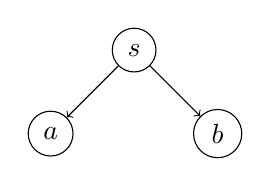
\begin{tikzpicture}[node distance={15mm},main/.style = {draw, circle}]
            \node[main] (s) {$s$};
            \node[main] (a) [below left of=s] {$a$};
            \node[main] (b) [below right of=s] {$b$};
            \draw[->] (s) -- (a);
            \draw[->] (s) -- (b);
        \end{tikzpicture}
    \end{center}
    We model the forwarding of the packet to the hosts with events
    $a$ and $b$ respectively.
    We can define the event structure with an empty conflict relation and the least enabling relation which satisfies:
    \begin{align*}
        \e \vdash_{min} a, \e \vdash_{min} b
    \end{align*}
    Assume that forwarding a packet to both hosts violates
    a safety property.
    Thus, we may consider the configuration $\sigma = \s{a,b}$ as
    a counterexample.
    In this example $\vec u$ is such that we have:
    \begin{align*}
         & CE(a,b) = false                   \\
         & ME(\e, a) = true, ME(\e,b) = true \\
    \end{align*}
    We have:
    \begin{align*}
        \varphi_{\sigma} & =
        \left(
        \left(
        E(\e, a) \wedge E(\s{a},b)
        \right)
        \vee
        \left(
        E(\e,b) \wedge E(\s{b},a)
        \right)
        \right)
        \wedge Con(\sigma)                                                       \\
        C(a,b)           & = CE(a,b)                                             \\
        M(\e, a)         & =  ME(\e,a) \wedge Min(\e, a) \wedge Con(\e)          \\
        M(\e, b)         & =  ME(\e,b) \wedge Min(\e, b) \wedge Con(\e)          \\
        M(\s{a}, b)      & =  ME(\s{a},b) \wedge Min(\s{a}, b) \wedge Con(\s{a}) \\
        M(\s{b}, a)      & =  ME(\s{b},a) \wedge Min(\s{b}, a) \wedge Con(\s{b}) \\
        E(\e, a)         & =  M(\e,a) \wedge Con(\e)                             \\
        E(\e, b)         & = M(\e,b) \wedge Con(\e)                              \\
        E(\s{a}, b)      & = (M(\s{a},b) \vee E(\e,b))\wedge Con(\s{a})          \\
        E(\s{b}, a)      & = (M(\s{b},a) \vee E(\e,a))\wedge Con(\s{b})          \\
        Con(\e)          & = true                                                \\
        Con(\s{a})       & = true                                                \\
        Con(\s{b})       & = true                                                \\
        Con(\s{a,b})     & = \neg C(a,b)                                         \\
        Min(\e, a)       & = \neg M(\s{b},a)                                     \\
        Min(\e, b)       & = \neg M(\s{a},b)                                     \\
        Min(\s{a}, b)    & = \neg M(\e, b)                                       \\
        Min(\s{b}, a)    & = \neg M(\e, a)                                       \\
    \end{align*}
    We consider an assignment to endogenous variables $\vec v$ for which we have:
    \begin{align*}
        (M,\vec v) & \vDash M(\e,a) = true       \\
        (M,\vec v) & \vDash M(\e,b) = true       \\
        (M,\vec v) & \vDash M(\s{a},b) = false   \\
        (M,\vec v) & \vDash M(\s{b},a) = false   \\
        (M,\vec v) & \vDash Min(\e,a) = true     \\
        (M,\vec v) & \vDash Min(\e,b) = true     \\
        (M,\vec v) & \vDash Min(\s{a},b) = false \\
        (M,\vec v) & \vDash Min(\s{b},a) = false \\
    \end{align*}
    Other variables do not have a cyclic dependency, thus their value
    can be uniquely determined in the context $\vec u$.
    Regarding this model and $\vec v$ we have:
    \begin{align*}
        (M,\vec v) \vDash (C(a,b) = false) \wedge \left(\varphi_{\sigma} = true\right)
    \end{align*}
    Now let's add a conflict between $a$ and $b$ so we manually set
    $C(a,b) = true$.
    Let $\vec v'$ be the new values of the endogenous variables
    after we have set $C(a,b) = true$.
    We have:
    \begin{align*}
        (M, \vec v') \vDash C(a,b) = true
        \Rightarrow  (M, \vec v') \vDash \neg \varphi_{\sigma}
    \end{align*}
    This means that there exists a solution to the equations in
    $M_{C(a,b) \leftarrow true}$ in the context $\vec u$ where we $\neg \varphi_{\sigma}$ holds.
    Thus we have:
    \begin{align*}
        (M, \vec u) \vDash \langle C(a,b) \leftarrow true \rangle \neg \varphi_{\sigma}
    \end{align*}
    Since we have considered the witness $(\emptyset, \emptyset, true)$
    and the set $\vec W$ in the witness is empty, we can conclude
    that $C(a,b) = true$ is a but-for cause for $\varphi_{\sigma}$
    in $(M,\vec u)$.
\end{example}

\begin{example}
    Consider a firewall where we initially allow all outgoing packets and block all incoming packets.
    We want to allow incoming packets once a packet is sent outside.
    So, we consider an event structure with events $i,o$ for incoming and
    outgoing packets respectively.
    We assume an empty conflict relation and enabling relation
    the least one that satisfies
    \begin{align*}
        \e \vdash i, \e \vdash o
    \end{align*}
    Then we can achieve a configuration $\sigma = \s{o}$ as a
    counterexample.
    We have:
    \begin{align*}
        \varphi_{\sigma} & = E(\e, o) \wedge Con(\s{o})
        = E(\e, o)
        \\
        CE(i,o)          & = false                                             \\
        ME(\e, i)        & = true                                              \\
        ME(\e, o)        & = true                                              \\
        ME(\s{i}, o)     & = false                                             \\
        ME(\s{o}, i)     & = false                                             \\
        E(\e, o)         & = M(\e,o) \wedge Con(\e)
        = M(\e, o)                                                             \\
        M(\e, o)         & = ME(\e,o) \wedge Min(\e, o)\wedge Con(\e)          \\
                         & = ME(\e,o) \wedge Min(\e, o)                        \\
        M(\s{i},o)       & = ME(\s{i},o) \wedge Min(\s{i},o) \wedge Con(\s{i}) \\
                         & = ME(\s{i},o) \wedge Min(\s{i},o)                   \\
        Min(\e, o)       & = \neg M(\s{i},o)                                   \\
        Min(\s{i},o)     & = \neg M(\e,o)
    \end{align*}
    Consider a $\vec v$ where:
    \begin{align*}
        M(\e, o)      & = true  \\
        Min(\e, o)    & = true  \\
        Min(\s{i}, o) & = false \\
        M(\s{i}, o)   & = false \\
    \end{align*}
    Thus we have:
    \begin{align*}
        (M,\vec v) \vDash (M(\s{i},o) = false)  \wedge \varphi_{\sigma}
    \end{align*}
    Now assume that we set $M(\s{i},o)$ to $true$.
    This will cause $Min(\e,o)$ and subsequently $M(\e,o)$ becomes false.
    Since we have $\varphi_{\sigma} = E(\e,o) = M(\e,o)$, so
    $\varphi_{\sigma}$ becomes false too.
    Consider $\vec v'$ as the new values of variables after our
    intervention.
    So we have:
    \begin{align*}
        (M,\vec v')\vDash M(\s{i},o) = true
        \Rightarrow
        (M,\vec v) \vDash \neg \varphi_{\sigma}
    \end{align*}
    So we have found a solution $\vec v'$ to the equations in
    $M_{M(\s{i},o)\la true}$ in the context $\vec u$ where $\neg \varphi_{\sigma}$ holds.
    Thus we have:
    \begin{align*}
        (M,\vec u) \vDash \langle M(\s{i},o) \la true \rangle \neg \varphi_{\sigma}
    \end{align*}
    Again, like the previous example, we have considered an empty $\vec W$, thus $M(\s{i},o)$ is a but-for cause for $\varphi_{\sigma}$ in $(M,\vec u)$.
\end{example}


\pagebreak
\begin{appendices}
    \section{Semantic Derivation of the Example\protect\footnote[1]
      {The source code of the tool that is used to
          generate this derivation is available here:
          \href{https://github.com/seyhani/estrest}
          {https://github.com/seyhani/estrest}
      }
     }
    % \import{./}{proof.tex}
\end{appendices}

\end{document}